\documentclass[28pt]{article}
\usepackage[OT1,OT2]{fontenc}
\usepackage[utf8]{inputenc}
\usepackage[english,bulgarian]{babel}
\usepackage{lmodern}
\usepackage{hyperref}
\usepackage{url}
\usepackage{graphicx}

\usepackage{geometry}
\geometry{left=3cm,right=1cm,top=1cm,bottom=3cm}

\usepackage{xcolor}
\usepackage{pgf,tikz}
%\usetikzlibrary{calc}
\usepackage{amssymb,amsmath,array,bm}
\usepackage[T1]{fontenc}
\usepackage[utf8]{inputenc}
\usepackage{hyperref}
\usepackage{multicol}
\usepackage{tabularx}
%opening
\title{}
\author{}

\hypersetup{
	colorlinks,
	linkcolor={black},
	citecolor={black},
	urlcolor={black}
}

\begin{document}
 

\includegraphics[width=0.9\textwidth]{logo} \\

\begin{center}
		СЕДЕМНАДЕСЕТА УЧЕНИЧЕСКА КОНФЕРЕНЦИЯ УК’17 \\ \vspace{3cm}
		ТЕМА НА ПРОЕКТА\\
		\large{Система за управление на обучението}\\ \vspace{3cm}
		Автори:\\
		Алекс Иванов Цветанов (8-ми клас) \\ и \\ Димо Димов Чанев (9-ти клас)\\
		СМГ, София\\ \vspace{3cm}

		Научени ръководители (консултанти): \\
		Красен Фердинандов и Васил Тинчев
\end{center}

\newpage
\tableofcontents
\newpage
\begin{abstract}
	\large{
  	Факт е, че има създадени вече системи за управление на обученията. Те имат някои недостатъци. Например: видеата на уроците са с продължителност 3-4 часа - твърде много; повечето системи нямат практически задачи за упражнение (програмиране се учи най-добре с практика, която липсва); други системи имат само теоретични тестове (напълно достатъчно за добро усвояване на знанията), но така не се отчитат практическите умения.
	
	Идеята на нашия проект е да направим онлайн система за управление на обученията, която да съчетава добри практики при организиране на уроците, така че да е интересно, полезно и максимално улеснено за обучаващия се. Най-важната част на проекта ни е да стимулираме бъдещия програмист, като му покажем, че не е толкова трудно, колкото звучи. Това става чрез онлайн състезания, насочени към неговото ниво, със сертификати и награди за най-добрите.
	
	Проектът ни е предназначен главно за начинаещи и по-напреднали в програмирането. Състезанията ще съдържат теоретична част, но най-вече ще бъдат ориентиране към практиката.
	
	Системата за теставане на практическите задачи е „\foreignlanguage{english}{The Judgata}“, отделен проект, който ние интегрираме в нашия.
	
	В този проект се включват и нашите преподаватели Делян Пирински, Краси Паскалев, Красен Фердинандов и Васил Тинчев.
}
\end{abstract}
\newpage
\section{Увод}
	Нашия проект представлява онлайн система за управление на обученията, която да съчетава най-добрите практики при организиране на уроците, така че да е интересно, полезно и максимално улеснено за обучаващия се. Най-важното в проекта ни е да поощряваме бъдещия програмист, като му демонстрираме, че не е толкова трудно, колкото звучи. Това става чрез онлайн състезания, насочени към неговото ниво, със сертификати и награди за най-добрите. \\
\\
	Проектът ни е предназначен за начинаещи и по-напреднали в програмирането. Състезанията ще съдържат теоретична част, но най-вече ще бъдат ориентиране към практиката. \\
\\
	Системата за теставане на практическите задачи е „\foreignlanguage{english}{The Judgata}“, отделен проект, който ние интегрираме в нашия. \\\vspace{0.5cm}
	
	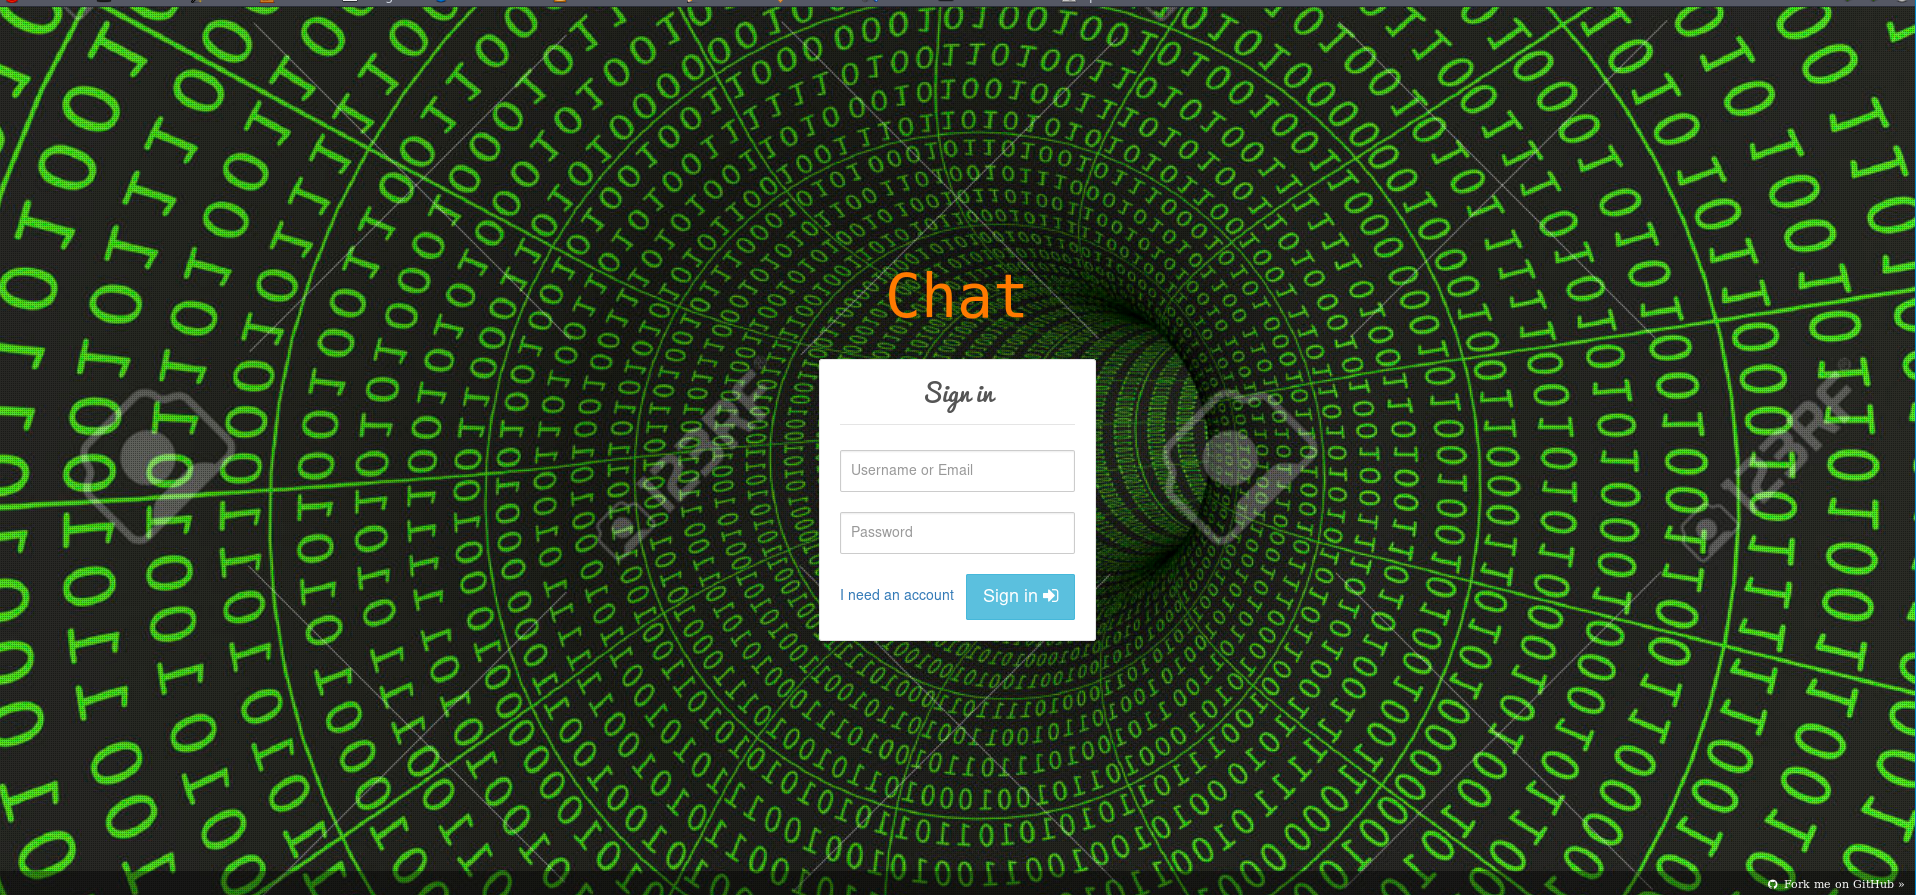
\includegraphics[width=0.9\textwidth]{chat} \\
	\newpage
	\section{Описание на реализацията}
	Схемата по-долу демонстира отделните части на приложението и връзките между тях:\\ \vspace{0.5cm} \\
	{\small
		\begin{tikzpicture}[
		auto,
		level 1/.style={sibling distance=50mm},
		level 2/.style={sibling distance=25mm},
		level 3/.style={sibling distance=25mm},
		level 4/.style={sibling distance=25mm},
		every node/.style = {shape=rectangle,
			draw, align=center,
			top color=white, bottom color=blue!20}]
		\node[draw] {Приложение}
		child
		{
			node[draw] {Ученическа система}
			child
			{
				node[draw] {Статична част}
				child
				{
					node[draw] {Секция\\„Курсове“}
				}
				child
				{
					node[draw] {Секция\\„Видеа“}	
				}
				child
				{
					node[draw] {Секция\\„Презентации“}	
				}
			}
			child
			{
				node[draw] {База данни}
			}
			child
			{
				node[draw] {Сертификати}
			}
		}
		child
		{
			child
			{
				node[draw,top color=white, bottom color=green!20] {\foreignlanguage{english}{The Jugdata}}
				child 
				{
					node[draw] {База данни}
				}
			}
		}
		child
		{
			node[draw] {Чат/Форум}
			child 
			{
				node[draw] {База данни}
			}
			child
			{
				node[draw] {Стаи}
			}
		}
		;
		\end{tikzpicture}
	}
	\\\vspace {2cm} \\
	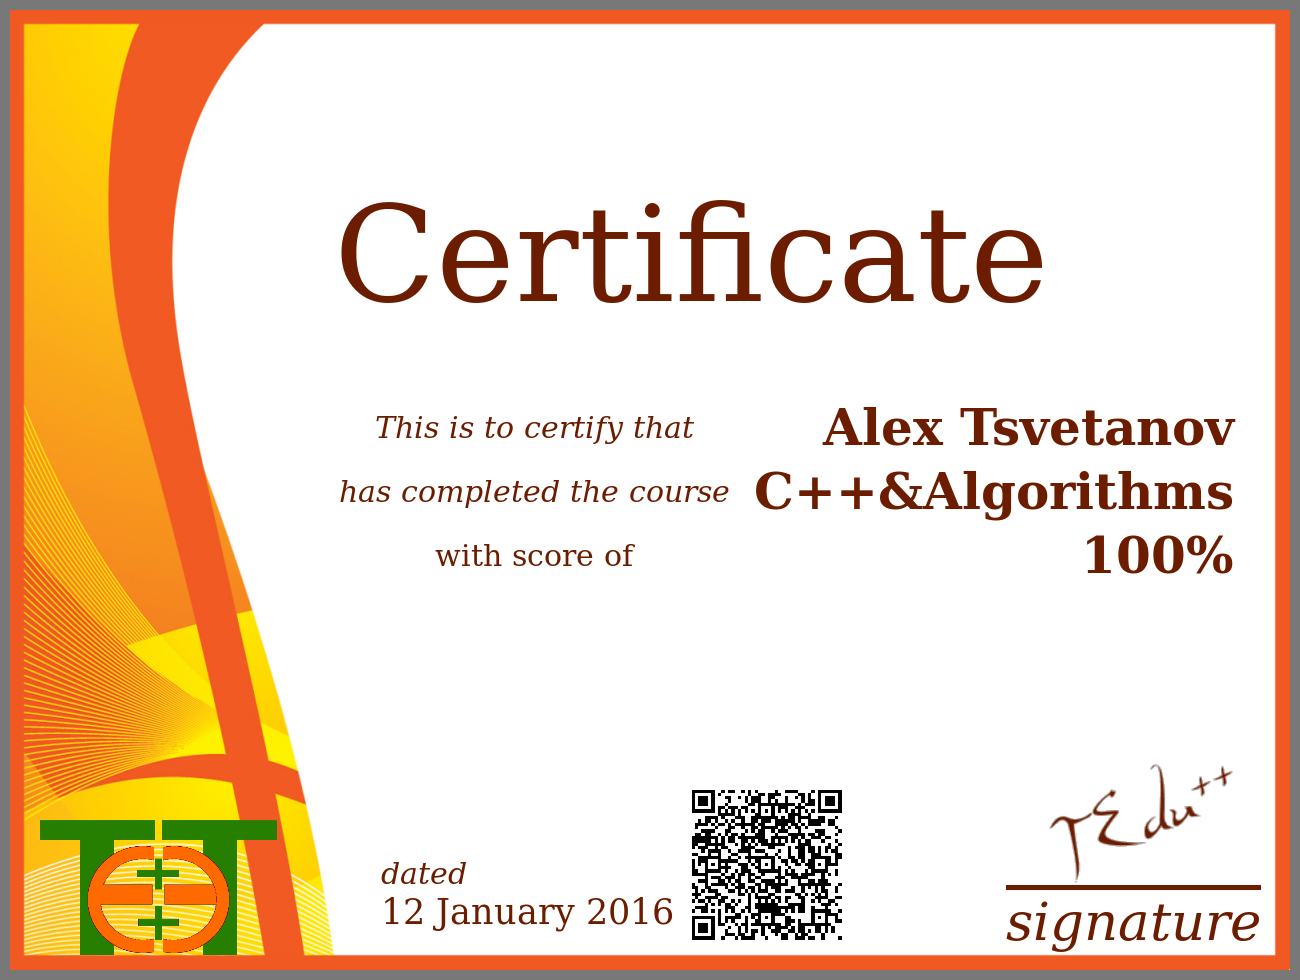
\includegraphics[width=0.9\textwidth]{cert} \\
	\newpage
	\section{Избор на програмно-технически средства}
	Технологиите, които използваме са добре известни и са се доказали с времето. Те са:
	\begin{itemize}
		\item \foreignlanguage{english}{NGINX} сървър
		\item \foreignlanguage{english}{Node.JS \& MongoDB} (\foreignlanguage{english}{The Judgata})
		\item \foreignlanguage{english}{JADE} (\foreignlanguage{english}{The Judgata})
		\item \foreignlanguage{english}{Reveal.JS} - инструмент за създаване на презентации
		\item \foreignlanguage{english}{Bootstrap (Jumbotron)}
		\item \foreignlanguage{english}{FastCGI - Fast Common Gateway Interface, C++, MySQL} (ученическа система)
	\end{itemize}
	\vspace{1cm}
	На \foreignlanguage{bulgarian}{с}хемата по-долу виждате отделните  части на приложениетf заедно със съответната технология:\\
	\vspace{0.5cm} \\
	{\small
	\begin{tikzpicture}[
	auto,
	level 1/.style={sibling distance=50mm},
	level 2/.style={sibling distance=25mm},
	level 3/.style={sibling distance=25mm},
	level 4/.style={sibling distance=25mm},
	every node/.style = {shape=rectangle,
		draw, align=center,
		top color=white, bottom color=blue!20}]
	\node[draw] {Приложение}
	child
	{
		node[draw] {Ученическа система}
		child
		{
			node[draw] {Статична част}
			child{child
			{
				node[draw,top color=white, bottom color=red!20] {\foreignlanguage{english}{Bootstrap}\\ \foreignlanguage{english}{(Jumbotron)}}
				child
				{
					node[draw] {Секция\\„Курсове“}
				}
				child
				{
					node[draw] {Секция\\„Видеа“}	
				}
			}}
			child
			{
				node[draw,top color=white, bottom color=red!20] {\foreignlanguage{english}{Reveal.JS}}
				child
				{
					node[draw] {Секция\\„Презентации“}	
				}
			}
		}
		child
		{
			node[draw] {База данни}
		}
		child
		{
			node[draw] {Сертификати}
		}
	}
	child
	{
		child
		{
			node[draw,top color=white, bottom color=green!20] {\foreignlanguage{english}{The Jugdata}}
			child 
			{
				node[draw,top color=white, bottom color=red!20] {\foreignlanguage{english}{Node.JS}}
				child
				{
					node[draw] {База данни}
					child
					{
						node[draw,top color=white, bottom color=red!20] {\foreignlanguage{english}{MongoDB}}	
					}	
				}
				child
				{
					node[draw] {Външен вид}
					child
					{
						node[draw,,top color=white, bottom color=red!20]{\foreignlanguage{english}{JADE}}	
					}	
				}
			}
		}
	}
	child
	{
		node[draw] {Чат/Форум}
		child 
		{
			node[draw,top color=white, bottom color=red!20] {\foreignlanguage{english}{Node.JS}}
			child
			{
				node[draw] {База данни}
				child
				{
					node[draw,top color=white, bottom color=red!20] {\foreignlanguage{english}{MongoDB}}	
				}	
			}
			child
			{
				node[draw] {Стаи}
			}
		}
	}
	;
	\end{tikzpicture}
}
\newpage
\section{Описание на програмната система/програмното осигуряване} 
Тъй като в проекта ни се налага дя работим с пароли за потребителите, използваме някой алгоритми за хеширане. \\ \vspace {0.5cm}
%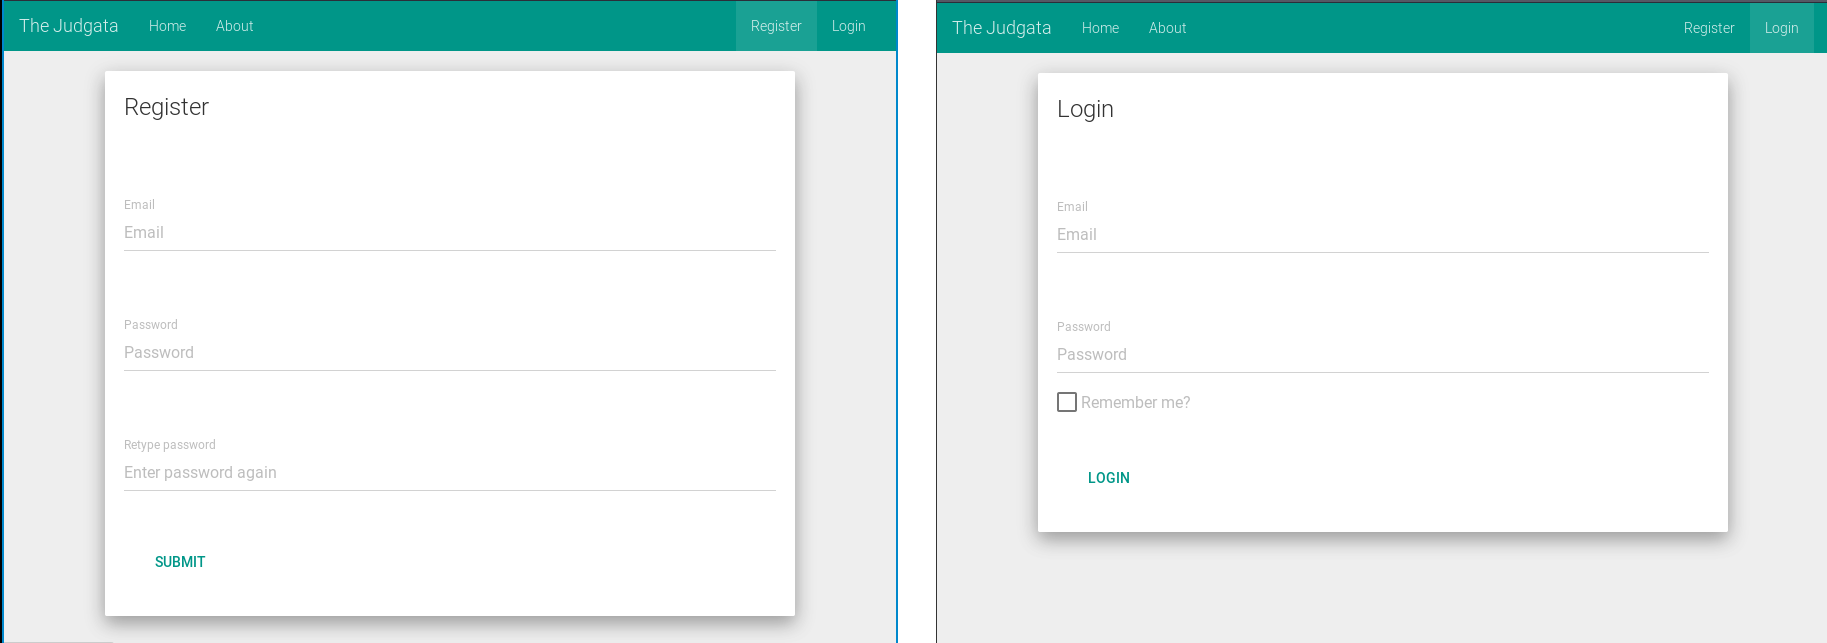
\includegraphics[width=1\textwidth]{logandreg} \\ \vspace {0.5cm}
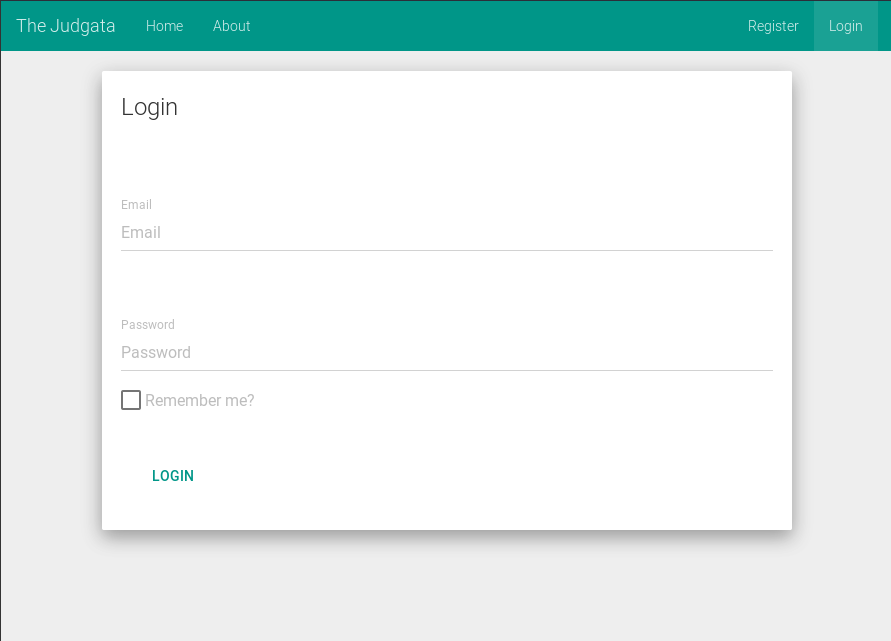
\includegraphics[width=0.85\textwidth]{login} \\ \vspace {0.5cm}
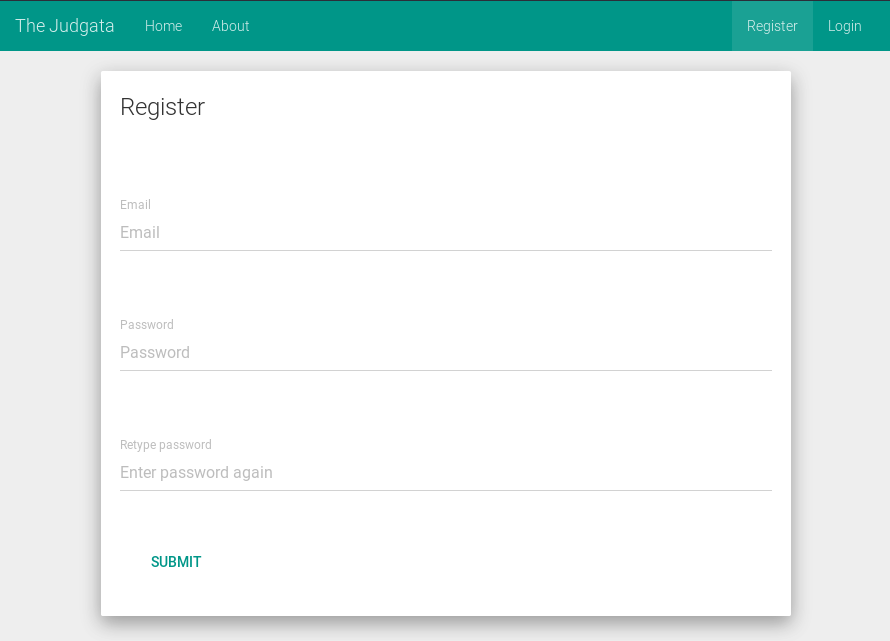
\includegraphics[width=0.85\textwidth]{register}
\newpage
\section{Защо този проект е по-добър от вече създадени такива?}
\begin{table}[ht]
	\centering
	\resizebox{\textwidth}{!}
	{
		\begin{tabular}{c|c|c|c}
			 & \foreignlanguage{english}{Telerik Academy by Progress} & Уча.се & Този проект\\
			\hline
			Продължителност & & & \\ 
			на & 3-4 часа & 3-4-5 минути & 10-12-15 минути \\ 
			един урок & & &\\
			 & & &\\
			\hline
			 & & &\\
			Практически задачи & Да & Не & Да \\ 
			 & & &\\
			\hline
			 & & &\\
			Теоретични задачи & Да & Да & Да \\ 
			 & & &\\
			\hline
			 & & &\\
			Безплатни ресурси & Само практическите задачи & Не & Да \\ 
			 & & &\\
			\hline
			 & & &\\
			 Издаване на сертификати & Да & Не & Да \\
			 & & &\\
			 \hline
			 & & &\\
			Възможност за & & & \\ 
			индивидуална работа с & Не & Не & Да \\
			обучаващия се & & &\\ 
			\hline
			
		\end{tabular}
	}
\end{table}
\newpage
\section{Изложение}
Нашия проект представлява онлайн система за управление на обученията, която да съчетава най-добрите практики при организиране на уроците, така че да е интересно, полезно и максимално улеснено за обучаващия се. Най-важното в проекта ни е да поощряваме бъдещия програмист, като му демонстрираме, че не е толкова трудно, колкото звучи. Това става чрез онлайн състезания, насочени към неговото ниво, със сертификати и награди за най-добрите. \\\vspace {3cm} \\
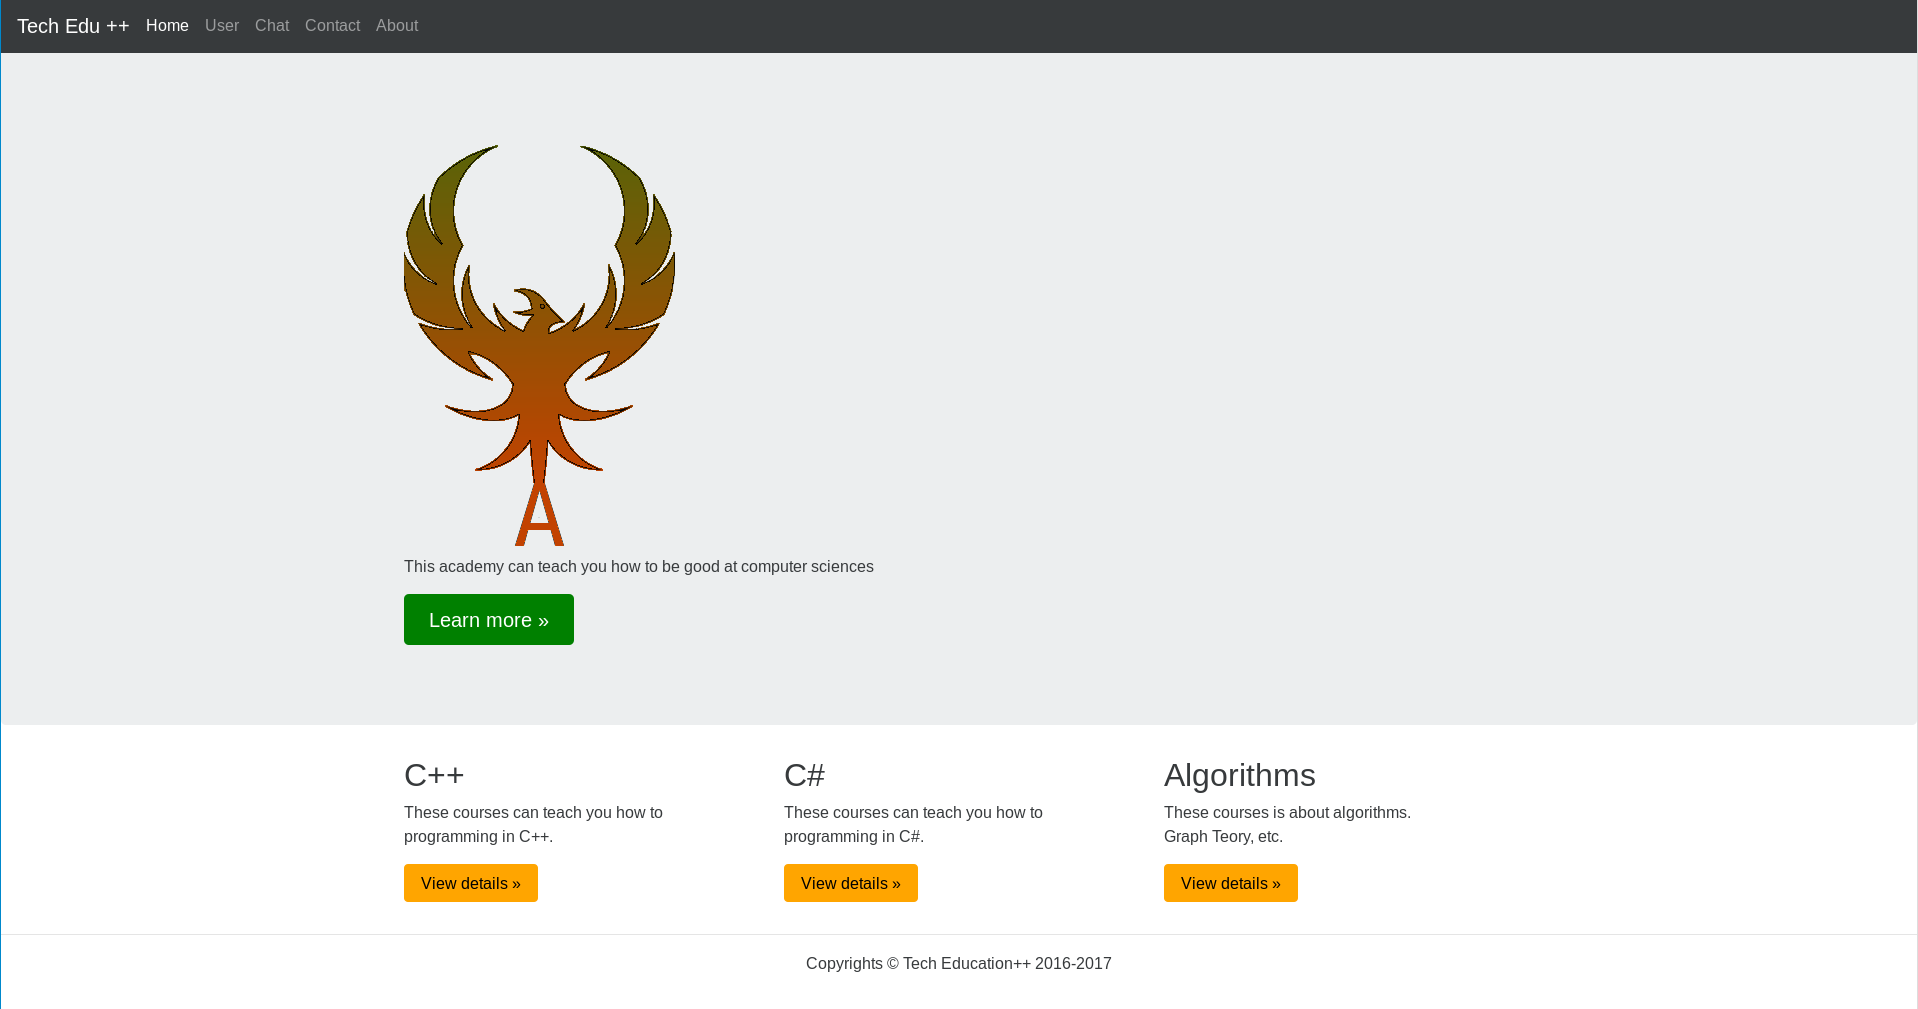
\includegraphics[width=0.9\textwidth]{academy} \\
\section{Преглед на проекта}
Може да прегледате проекта \href{https://infocourse.techedu.cf}{тук} 
\section{Информация за участниците в него}
Може да прегледате участниците в проекта \href{https://techedu.cf}{тук} 
\section{Информация за \foreignlanguage{english}{The Judgata}}
Може да прегледате  в проекта \href{https://judge.techedu.cf}{тук} 
\newpage
\section{Благодарности}
Специални благодарности на:
\begin{itemize}
	\item Мария-Йоанна Александрова за добрите идеи за дизайн
\end{itemize}
Благодарности също за:
\begin{itemize}
	\item УчИМИ - Ученически Институт по Математика и Информатика
	\item БАН - Българска Академия на Науките
	\item СМГ - Софийска Математическа Гимназия
\end{itemize}
\selectlanguage{english}
\begin{thebibliography}{99}
\foreignlanguage{english}{
	\bibitem{reaveal}
	{\itshape Reveal.JS}.
	\texttt{http://lab.hakim.se/reveal-js/}. \\
	Copyright \copyright\; 2016 Hakim El Hattab. All rights reserved.
	\bibitem{judgata}
	{\itshape The Judgata}.
	\texttt{https://judge.techedu.cf/}. \\
	Copyright \copyright\; 2007 Free Software Foundation, Inc. All rights reserved.
	\bibitem{dom-to-image}
	{\itshape DOM to image}.
	\texttt{https://github.com/tsayen/dom-to-image}. \\
	Copyright \copyright\; 2015 Anatolii Saienko
	\bibitem{letschat}
	{\itshape Let's chat}.
	\texttt{https://github.com/sdelements/lets-chat}. \\
	Copyright \copyright\; 2012-2015 Houssam Haidar
	\bibitem{latex}
	{\itshape \LaTeX}.
	\texttt{https://www.latex-project.org/}.
}
\end{thebibliography}


\end{document}
